\documentclass[dvipdfmx, tikz]{standalone}
\usepackage{tikz}
\usetikzlibrary{calc,decorations.pathreplacing,quotes,positioning,shapes,fit,arrows,backgrounds,tikzmark}

\begin{document}
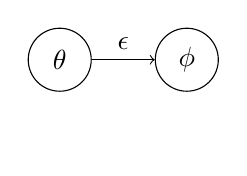
\begin{tikzpicture}[state/.style={circle, draw, minimum size=.8cm}, node distance=.8cm]
	\node(a0) [state] at (0,0) {$\theta$};
	\node(a1) [state, right =of a0] {$\phi$};
  \node(phantom) at (0,-1) {};
	
  \draw [->] (a0) to node(e0)[midway, above] {$\epsilon$} (a1);
  \ifx\TNFAActivateEdgeLabel\undefined \else
    \node[below=.2 of e0] {$p\mathchar`-edge$};
  \fi
\end{tikzpicture}
\end{document}
